Cases are taken from the demo band of D4 (4096$\times$2621\,px, look direction 1 on 97\,\% of
the SAR), the same band the Gate~3 jobs ran on. Every model is run through the worker
pipeline, once on the clear band and once with a synthetic 50\,\% cloud cover (study S3
generator, fixed seed). The band is cut into 256\,px windows (128\,m), and each case is the
window that best meets a measured criterion; none is picked by eye
(\texttt{scripts/gallery.py}, statistics in \texttt{docs/figures/gallery.json}).
Figures~\ref{fig:success} and~\ref{fig:failure} colour true positives blue, false positives
orange and missed building pixels yellow.

Over the whole band, pixel IoU is optical 0.734, SAR 0.536 and fused 0.712 on clear imagery.
Under the 50\,\% cloud cover it is 0.629 for the cloud-trained optical model, 0.619 for
cloud-trained fused, and 0.129 for the clean-trained optical model.

\begin{figure}[p]
\centering
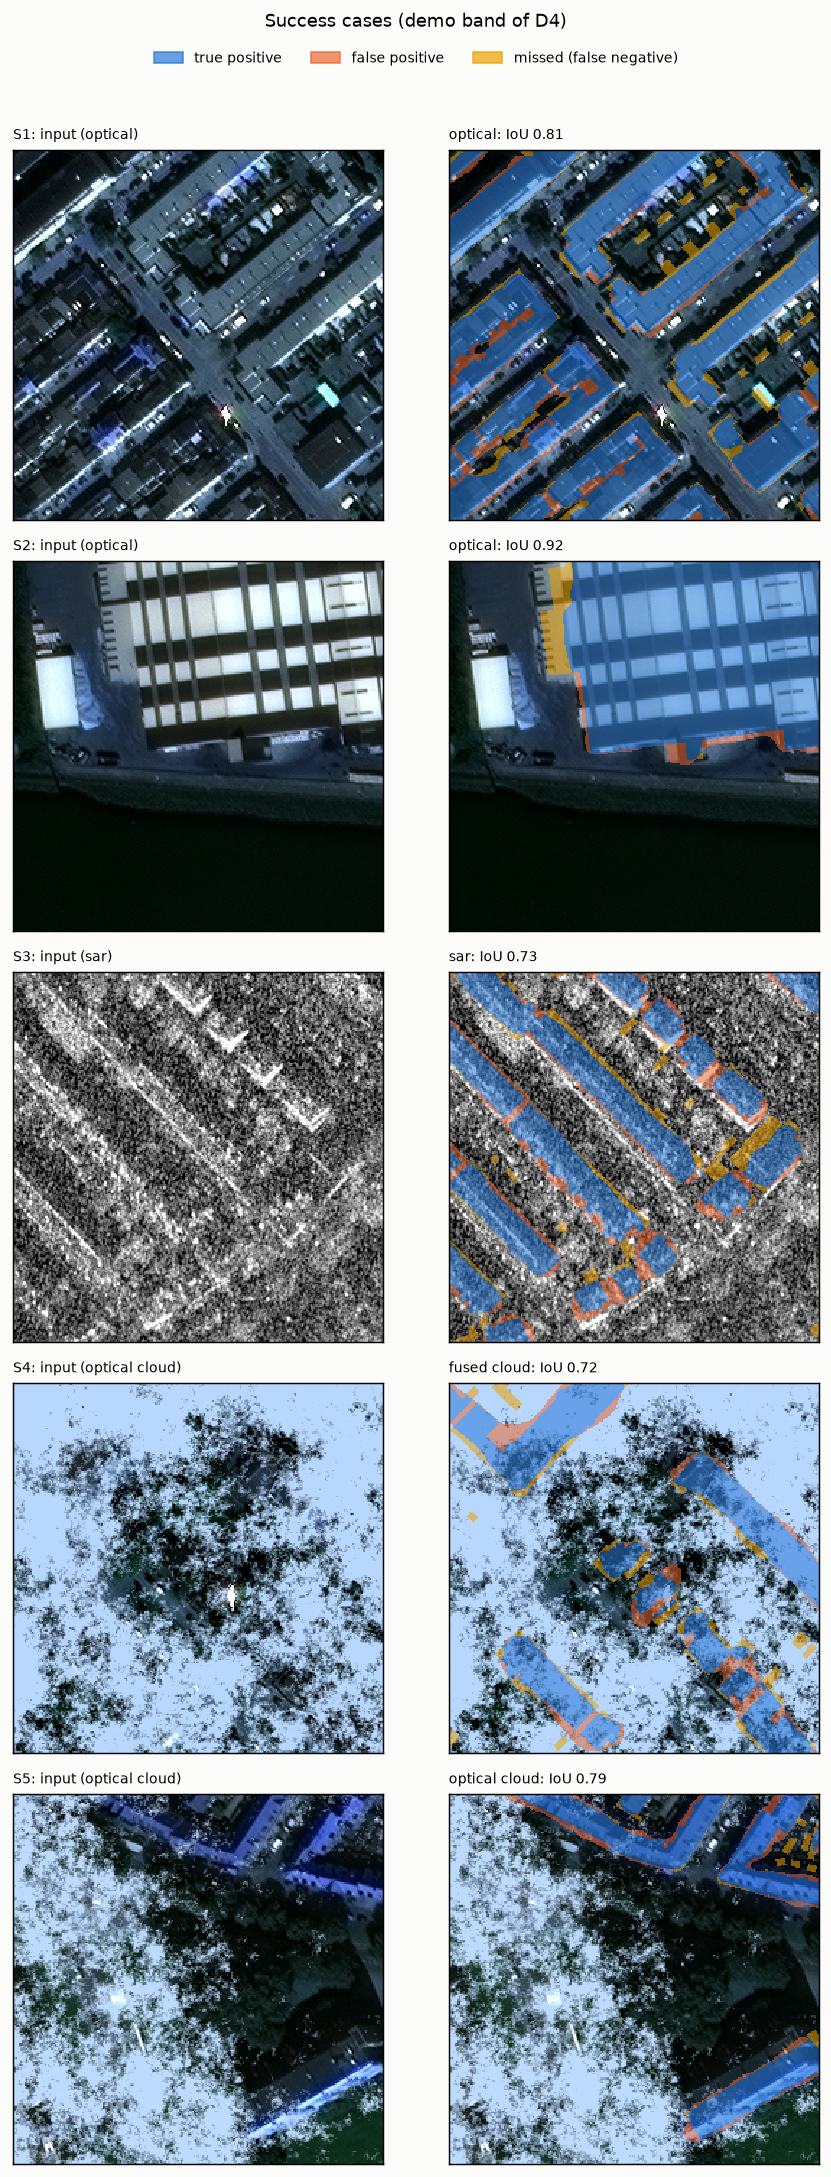
\includegraphics[height=0.92\textheight]{gallery_success.png}
\caption{Success cases S1--S5.}
\label{fig:success}
\end{figure}

\begin{figure}[p]
\centering
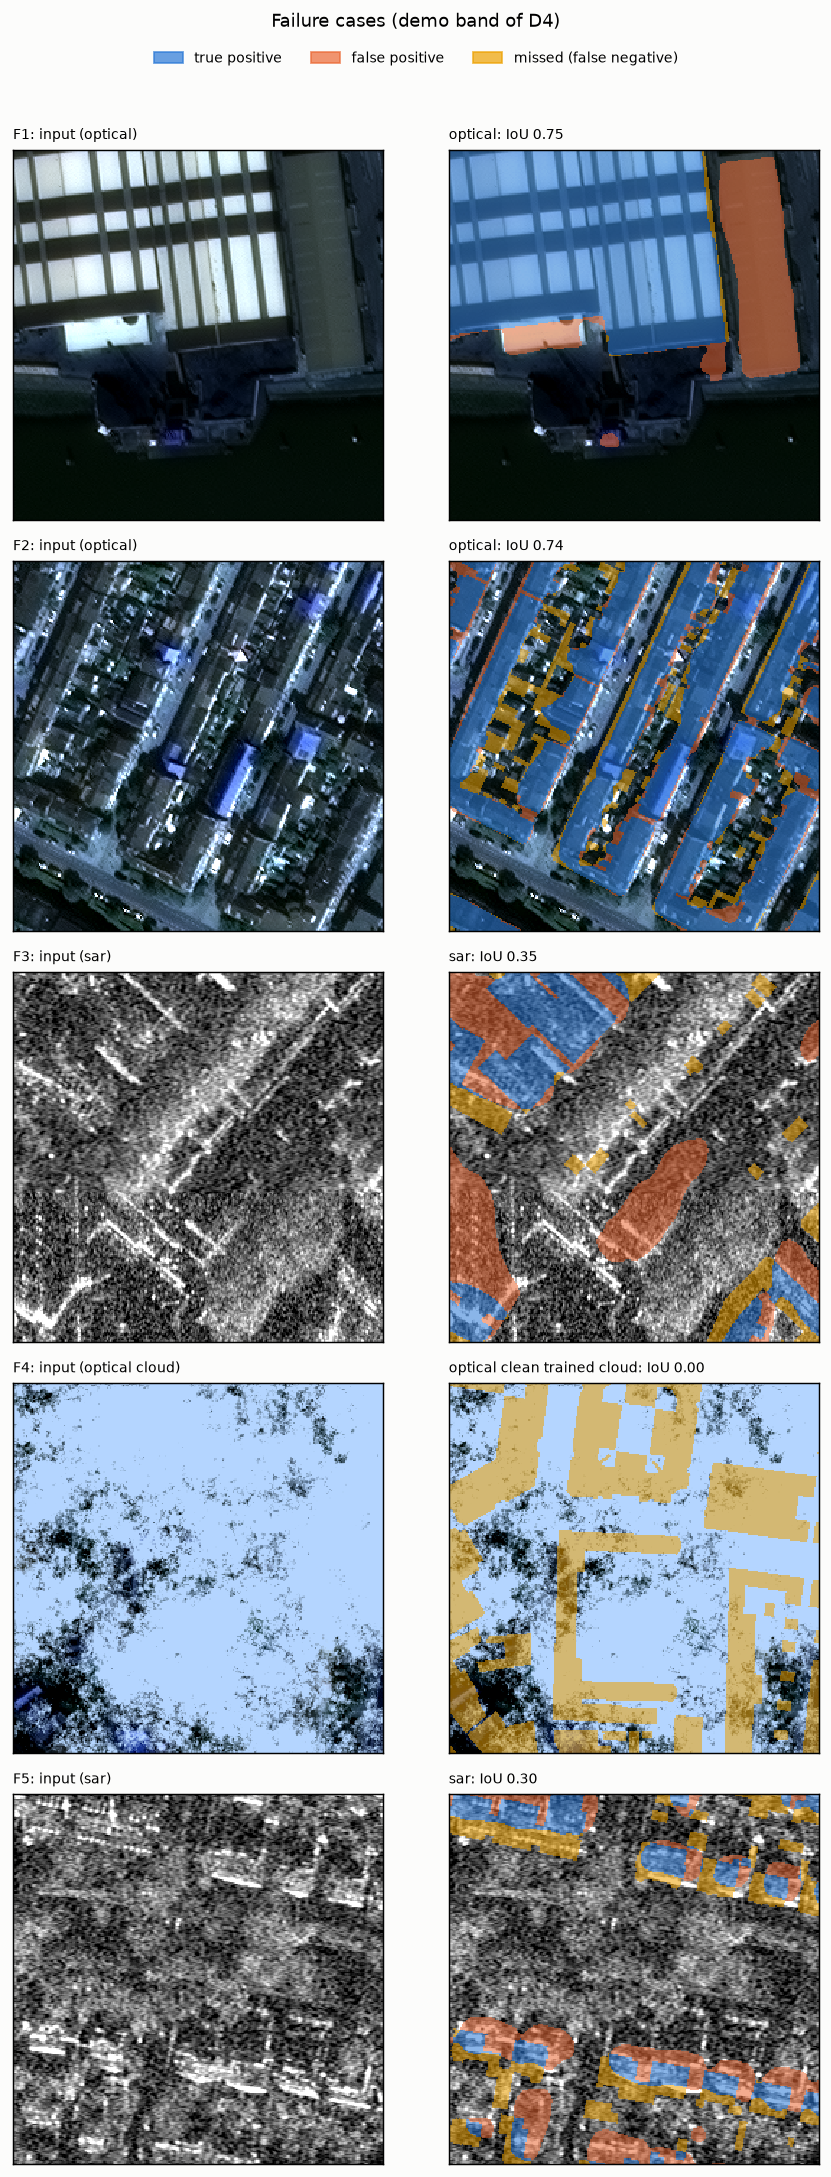
\includegraphics[height=0.92\textheight]{gallery_failure.png}
\caption{Failure cases F1--F5.}
\label{fig:failure}
\end{figure}

\subsection*{Success cases}
\begin{description}
\item[S1 Dense residential block (optical, IoU 0.81).] Twenty-three terraced houses fill
44\,\% of the window. Roof outlines follow the footprints; the errors are a one- to two-pixel
rim along the street edges (orange) and back extensions missed in the shadow of the rows
(yellow). Morphological closing keeps each roof row in one piece, and the 4-connectivity
rule keeps rows that touch at a corner apart.
\item[S2 Large buildings (optical, IoU 0.92).] One industrial hall of 22\,500\,px
(5600\,m$^2$) with a strongly patterned roof is segmented as a single object, so the
skylight stripes are not mistaken for gaps. The only miss is a narrow strip at the hall's
west edge, where the roof is darker.
\item[S3 SAR only (IoU 0.73).] Long rows of houses produce bright double-bounce lines in
the SAR. Because every strip is flipped to the same look direction (D5), the model reads
the bright line and the shadow behind it consistently. Phase correlation finds no offset
between the SAR prediction and the footprints here (0.1, 0.2\,px), so the alignment is
correct.
\item[S4 Fused under cloud (IoU 0.72 vs 0.00).] Clouds cover 71\,\% of the window. The
clean-trained optical model finds nothing (IoU 0.00); the cloud-trained fused model still
recovers 0.72, close to its clear-sky 0.76, because the SAR channels carry the building
structure where the optical channels are white. This is the S3 result at the scale of one
neighbourhood.
\item[S5 Thin cloud, cloud-trained optical (IoU 0.79).] At 34\,\% cover, cloud augmentation
makes the optical model ignore haze and partial cloud: its IoU drops only from 0.81 to
0.79, against 0.70 for the clean-trained model on the same pixels.
\end{description}

\subsection*{Failure cases}
\begin{description}
\item[F1 False positives on a building-like structure (optical).] The window has one
labelled hall. The large orange area is a long, flat, roofed structure next to it (and a
small part of the quay apron) that is not in the label set, giving 7\,500 false-positive
pixels. From above it looks like a roof, but it is not in the labels; the SAR model
barely fires on it (57 false-positive pixels). Whether it is a missing label or a true
error cannot be told from the imagery alone, so this case mixes label ambiguity with model
error. Here the fused model does worse (IoU 0.42), so fusion did not learn to use the SAR
evidence in this case.
\item[F2 Adjacent buildings merged (optical, IoU 0.74).] Nineteen terraced houses with
narrow back yards. In 8 places one predicted component covers three or more labelled
buildings. Gaps of a few pixels between rows are filled by the network and by the
morphological closing, while small rear extensions are missed (yellow). Pixel IoU stays
high, but object F1 drops because one blob matches no single footprint at IoU $\ge 0.5$.
This is the main reason object F1 (0.50) is far below pixel F1 (0.81). Instance-aware
outputs (a boundary class or a distance transform with watershed) are the usual fix.
\item[F3 SAR false detections (IoU 0.35).] The SAR model marks two large blobs over an area
of textured, non-building backscatter (the orange shapes in the lower half) and
mis-places several real buildings. Phase correlation between the prediction and the
footprints finds no consistent shift (peak response 0.06), so this is not a clean layover
offset but bright clutter that looks like building returns. Trees and other rough
surfaces can give high, irregular returns in SAR, which despeckling reduces but does not
remove.
\item[F4 Clean-trained optical under heavy cloud (IoU 0.00).] At 85\,\% cover the
clean-trained model returns nothing for 26 buildings. Under the same clouds the
cloud-trained optical model reaches 0.40 and the fused model 0.47. The failure is the
model never having seen clouds in training, not the sensor alone.
\item[F5 SAR in a dense block (IoU 0.30).] Small houses (465\,px, 116\,m$^2$ on average)
packed in rows. Their double-bounce lines merge and the model outlines the bright lines
rather than the roofs, giving offset outlines and missed rear parts. This window shows the
known limit of SAR building mapping at 0.5\,m (shadow and layover of neighbouring
buildings overlap), and it is why the SAR-only object F1 stays at 0.24--0.26 whatever the
pre-processing.
\end{description}

\paragraph{Stitching seams} are a sixth, solved failure: Fig.~\ref{fig:s1} shows the hard
tile-corner edges of naive stitching that Hann blending removes (S1).
